% Options for packages loaded elsewhere
\PassOptionsToPackage{unicode}{hyperref}
\PassOptionsToPackage{hyphens}{url}
%
\documentclass[
  letterpaper,
  landscape]{article}
\usepackage{lmodern}
\usepackage{amssymb,amsmath}
\usepackage{ifxetex,ifluatex}
\ifnum 0\ifxetex 1\fi\ifluatex 1\fi=0 % if pdftex
  \usepackage[T1]{fontenc}
  \usepackage[utf8]{inputenc}
  \usepackage{textcomp} % provide euro and other symbols
\else % if luatex or xetex
  \usepackage{unicode-math}
  \defaultfontfeatures{Scale=MatchLowercase}
  \defaultfontfeatures[\rmfamily]{Ligatures=TeX,Scale=1}
\fi
% Use upquote if available, for straight quotes in verbatim environments
\IfFileExists{upquote.sty}{\usepackage{upquote}}{}
\IfFileExists{microtype.sty}{% use microtype if available
  \usepackage[]{microtype}
  \UseMicrotypeSet[protrusion]{basicmath} % disable protrusion for tt fonts
}{}
\makeatletter
\@ifundefined{KOMAClassName}{% if non-KOMA class
  \IfFileExists{parskip.sty}{%
    \usepackage{parskip}
  }{% else
    \setlength{\parindent}{0pt}
    \setlength{\parskip}{6pt plus 2pt minus 1pt}}
}{% if KOMA class
  \KOMAoptions{parskip=half}}
\makeatother
\usepackage{xcolor}
\IfFileExists{xurl.sty}{\usepackage{xurl}}{} % add URL line breaks if available
\IfFileExists{bookmark.sty}{\usepackage{bookmark}}{\usepackage{hyperref}}
\hypersetup{
  hidelinks,
  pdfcreator={LaTeX via pandoc}}
\urlstyle{same} % disable monospaced font for URLs
\usepackage[left=3.8cm,right=2.5cm,top=2.5cm,bottom=2.5cm]{geometry}
\usepackage{graphicx,grffile}
\makeatletter
\def\maxwidth{\ifdim\Gin@nat@width>\linewidth\linewidth\else\Gin@nat@width\fi}
\def\maxheight{\ifdim\Gin@nat@height>\textheight\textheight\else\Gin@nat@height\fi}
\makeatother
% Scale images if necessary, so that they will not overflow the page
% margins by default, and it is still possible to overwrite the defaults
% using explicit options in \includegraphics[width, height, ...]{}
\setkeys{Gin}{width=\maxwidth,height=\maxheight,keepaspectratio}
% Set default figure placement to htbp
\makeatletter
\def\fps@figure{htbp}
\makeatother
\setlength{\emergencystretch}{3em} % prevent overfull lines
\providecommand{\tightlist}{%
  \setlength{\itemsep}{0pt}\setlength{\parskip}{0pt}}
\setcounter{secnumdepth}{5}
\usepackage{amsmath} \usepackage{pdflscape} \usepackage{tikz} \usepackage{xcolor}
\newcommand{\blandscape}{\begin{landscape}} \newcommand{\elandscape}{\end{landscape}}
\newcommand{\bcenter}{\begin{center}} \newcommand{\ecenter}{\end{center}}

\author{}
\date{\vspace{-2.5em}}

\begin{document}

\begin{verbatim}
## # A tibble: 4,579 x 13
##    function_name calculator     N init_time calc_time calc_hz bytes max_error
##    <chr>         <chr>      <dbl>     <dbl>     <dbl>   <dbl> <dbl>     <dbl>
##  1 Smooth_exp    linear in~     8         0    4.83e7  20.7       8    0.484 
##  2 Smooth_exp    linear in~    12         0    8.27e7  12.1       8    0.356 
##  3 Smooth_exp    linear in~    16         0    1.95e8   5.13      8    0.226 
##  4 Smooth_exp    linear in~    20         0    4.09e8   2.45      8    0.134 
##  5 Smooth_exp    linear in~    24         0    7.33e8   1.36      8    0.151 
##  6 Smooth_exp    linear in~    28         0    1.31e9   0.764     8    0.140 
##  7 Smooth_exp    linear in~    32         0    2.19e9   0.457     8    0.0665
##  8 Smooth_exp    linear in~    36         0    3.39e9   0.295     8    0.0568
##  9 Smooth_exp    linear in~    40         0    5.01e9   0.200     8    0.0591
## 10 Smooth_exp    linear in~    44         0    7.27e9   0.138     8    0.0498
## # ... with 4,569 more rows, and 5 more variables: blank_column <lgl>,
## #   err1 <dbl>, err2 <dbl>, err3 <dbl>, Blank <lgl>
\end{verbatim}

\pagenumbering{roman}

\newpage

\%

\LARGE\{My Report or Thesis Title\} \%

\bigskip                \% \bigskip

\large\{Dr Hale\}

\newpage

\begin{center}

\large\{Abstract\}

\end{center}

\bigskip

\ldots this is the abstract text\ldots{}

\newpage

\tableofcontents

\newpage

\hypertarget{list-of-tables}{%
\section*{List of tables}\label{list-of-tables}}
\addcontentsline{toc}{section}{List of tables}

\renewcommand{\listtablename}{}

\listoftables

\newpage

\hypertarget{list-of-figures}{%
\section*{List of figures}\label{list-of-figures}}
\addcontentsline{toc}{section}{List of figures}

\renewcommand{\listfigurename}{}
\listoffigures

\newpage

\pagenumbering{arabic}

\hypertarget{intro}{%
\section{Introduction}\label{intro}}

\hypertarget{meths}{%
\section{Methods}\label{meths}}

\hypertarget{equations}{%
\subsection{Equations}\label{equations}}

This is an \(x=y\) equation.

\hypertarget{bullets}{%
\subsection{Bullets}\label{bullets}}

\hypertarget{res}{%
\section{Results}\label{res}}

\hypertarget{r-code-chunk}{%
\subsection{R-code chunk}\label{r-code-chunk}}

\hypertarget{r-code-inline}{%
\subsection{R-code inline}\label{r-code-inline}}

\hypertarget{images}{%
\subsection{Images}\label{images}}

\hypertarget{resultsFigs}{%
\subsection{Figures}\label{resultsFigs}}

\begin{figure}

{\centering 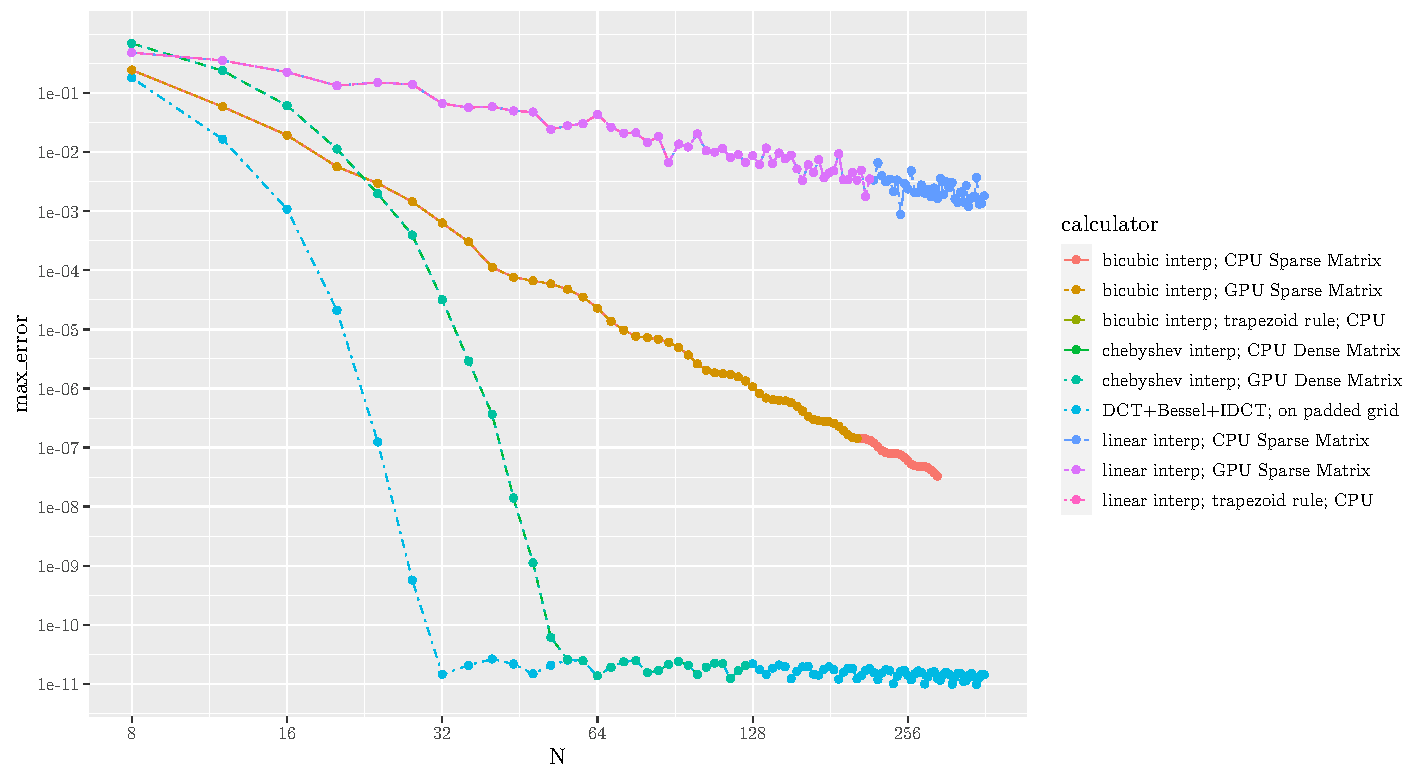
\includegraphics{myThesis_files/figure-latex/unnamed-chunk-3-1} 

}

\caption{Smooth Exp (Double)}\label{fig:unnamed-chunk-3}
\end{figure}

\begin{figure}

{\centering 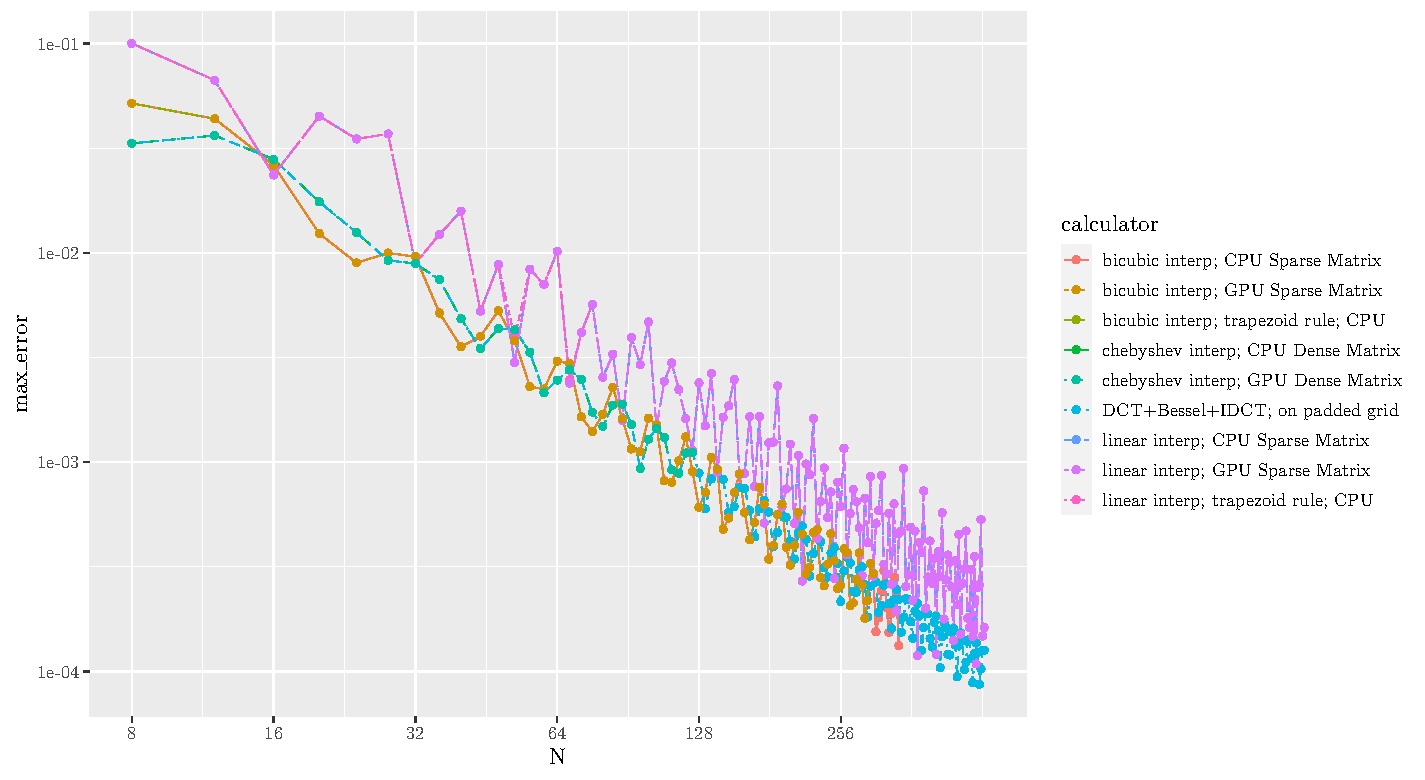
\includegraphics{myThesis_files/figure-latex/unnamed-chunk-4-1} 

}

\caption{Smooth Poly}\label{fig:unnamed-chunk-4}
\end{figure}

\begin{figure}

{\centering 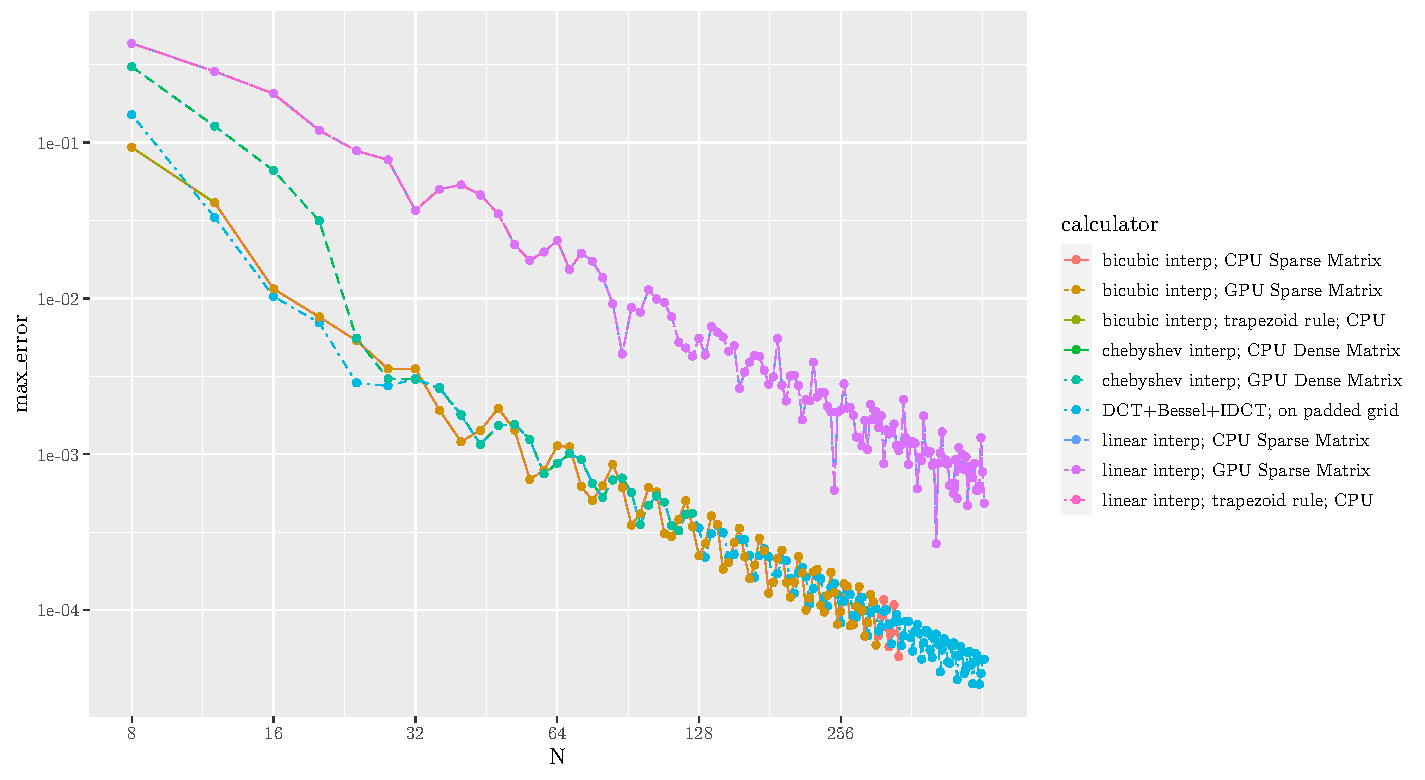
\includegraphics{myThesis_files/figure-latex/unnamed-chunk-5-1} 

}

\caption{Smooth Runge}\label{fig:unnamed-chunk-5}
\end{figure}

\begin{figure}

{\centering 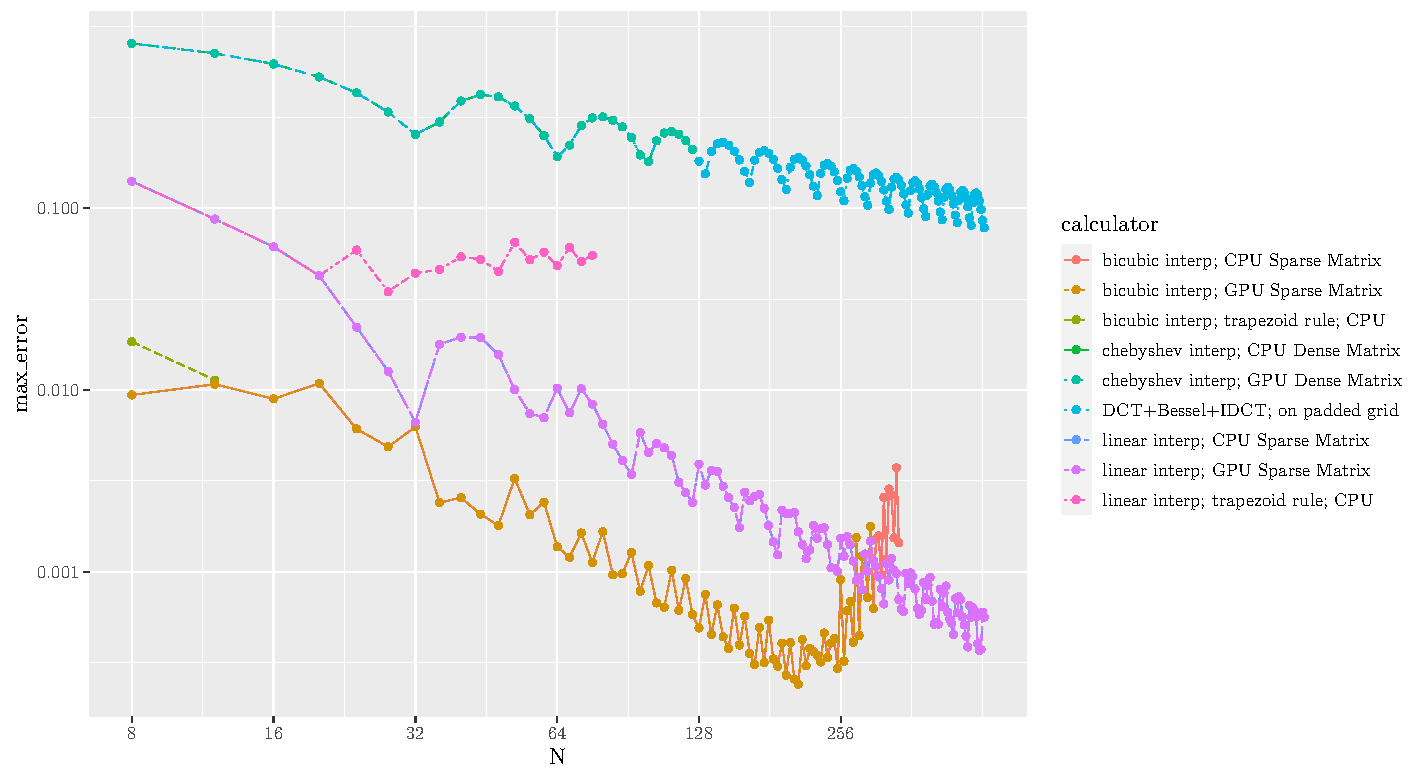
\includegraphics{myThesis_files/figure-latex/unnamed-chunk-6-1} 

}

\caption{Nonsmooth Sqrt}\label{fig:unnamed-chunk-6}
\end{figure}

\begin{figure}

{\centering 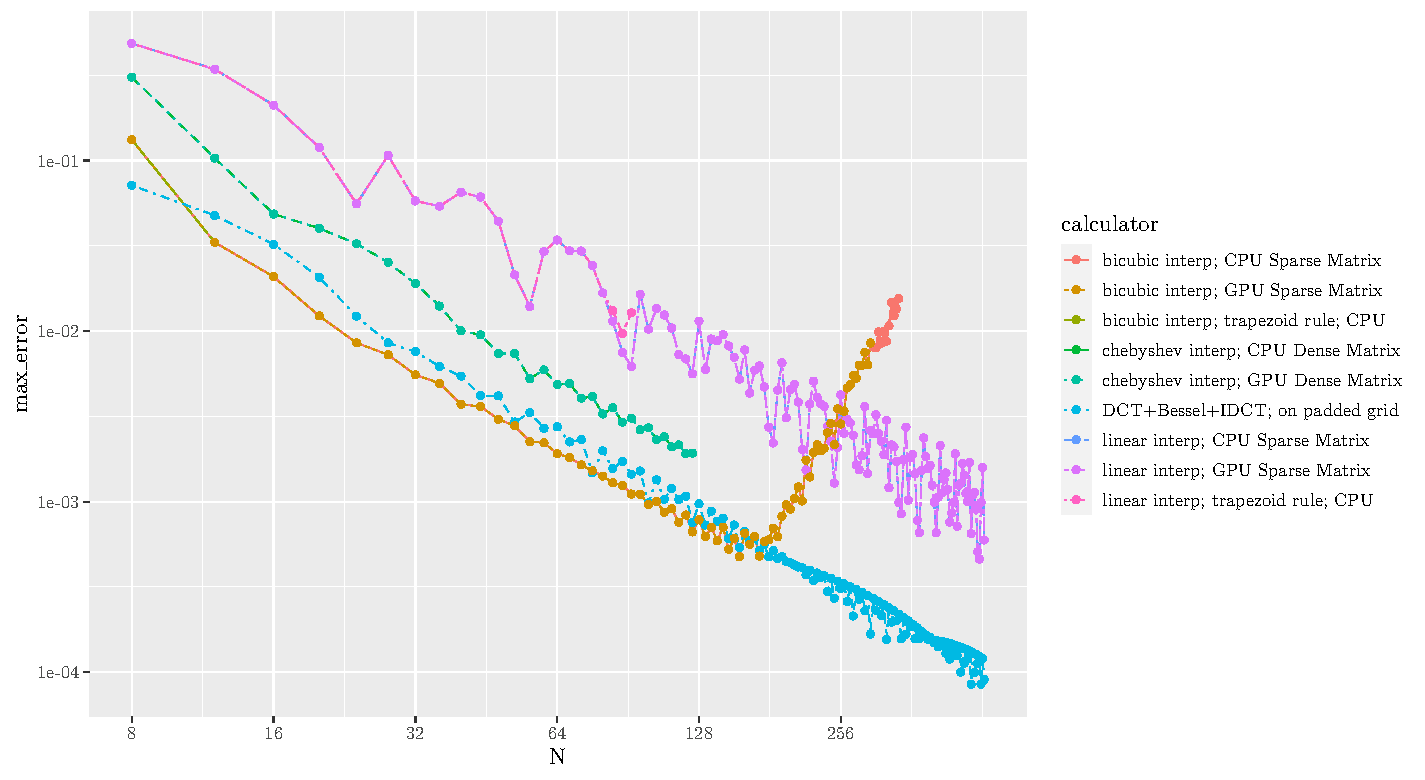
\includegraphics{myThesis_files/figure-latex/unnamed-chunk-7-1} 

}

\caption{Nonsmooth Abs}\label{fig:unnamed-chunk-7}
\end{figure}

\begin{figure}

{\centering 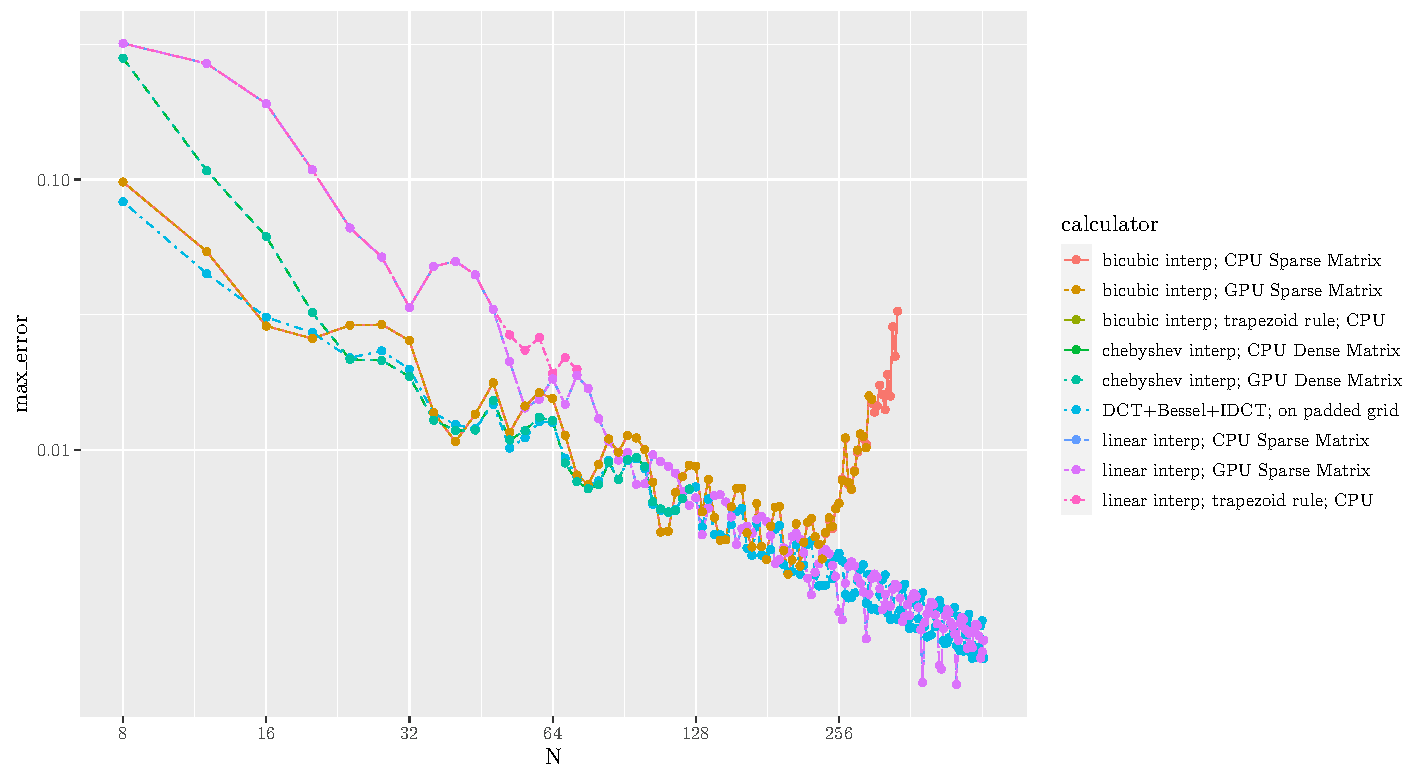
\includegraphics{myThesis_files/figure-latex/unnamed-chunk-8-1} 

}

\caption{NonSmooth Runge Abs}\label{fig:unnamed-chunk-8}
\end{figure}

\#\}

\hypertarget{resultsTables}{%
\subsection{Tables}\label{resultsTables}}

\hypertarget{con}{%
\section{Conclusion}\label{con}}

We described methods in Section \ref{meths} and plotted the results in
Section \ref{resultsFigs}. Supplementary material is in Appendix
\ref{app:mat}.

\hypertarget{references}{%
\section*{References}\label{references}}
\addcontentsline{toc}{section}{References}

\hypertarget{refs}{}

\renewcommand{\thesection}{\Alph{section}}
\setcounter{section}{1}

\hypertarget{appendix}{%
\section*{Appendix}\label{appendix}}
\addcontentsline{toc}{section}{Appendix}

\hypertarget{app:mat}{%
\subsection{Supporting material}\label{app:mat}}

\hypertarget{supporting-code}{%
\subsection{Supporting code}\label{supporting-code}}

\end{document}
